\documentclass[a4paper,12pt]{article}
\usepackage{a4wide}
\usepackage{acronym}
\usepackage{graphicx}
\usepackage{amssymb,amsmath}
\usepackage[title,titletoc,toc]{appendix}


\begin{document}

\begin{center}
{\LARGE\bf Travelling Thief Problem}\\
\vspace{0.5cm}
{\Large\bf Evolutionary Computation}\\
\vspace{1cm}
Prepared by William Reid, Matthew Hart, Samantha Peachey \& Alec Bellati\\
\vspace{1cm}
School of Computer Science,\\
The University of Adelaide\\
\vspace{1cm}
\today
\end{center}



\section*{Exercise 4}
In the planning phase, two algorithms were conceptualised that could potentially solve the Travelling Thief Problem. The first of these algorithms was based on the ``Ant Colony Optimisation'' method that was discussed in lectures. The second was an optimisation to the naive solution based on a recognised heuristic of the problem that taking items early in the tour is likely to be more expensive than taking items as late in the tour as possible.

% ALGORITHM 1

\subsection*{Algorithm 1: Ant Thieves}

The ant thieves (AT) algorithm is an ant colony optimization algorithm. The idea behind this approach is to try and optimise both the tour and knapsack at the same time unlike the approaches in exercise 2 and 3.


\subsubsection*{1. Setup}

At the start of the algorithm, each item and path is given an attractiveness and pheromone value. The attractiveness is a constant value which is used to determine how valuable the item or path is to take. The attractiveness of an item can be calculated by the following equation:

\begin{equation}
\frac{Weight}{Profit}
\end{equation}

The attractiveness of a path can be calculated by the following equation:

\begin{equation}
\frac{1}{Length}
\end{equation}

The pheromone value of the items and paths changes throughout the run of the algorithm and not at the constant rate aswell.

\subsubsection*{2. Find ant solutions}

AT uses “ants” which walk along paths between cities and sometimes picking up item(s) at the city visited. An equal amount of two types of ants are considered when finding solutions. One ant finds the tour first then fills its knapsack, while the other does the other way around.

\paragraph*{2a. Tour-first ant}

The tour-first ant finds a tour of between every city then uses this route to determine which items it should take.

Starting from the first city, the ant calculates a probability to take each path by considering the attractiveness and pheromone value of it. The probability for some path x can be calculated using the following formula where n is the number of paths being considered:

\begin{equation}
\frac{Attractiveness_{x} * Pheromone_{x}}{\sum_{i = 1}^{n} Attractiveness_{i} * Pheromone_{i}}
\end{equation}

The ant repeats this set with each time not considering the previous city until the entire path has been found.

Afterwards the ant picks up items by starting considering them starting from the back of the tour. The probability that an item x will be taken is the following:

\begin{equation}
\frac{Pheromone_{x}}{Pheromone_{MAX}}
\end{equation}

The ant stops picking up items when the next item considered will not fit in its knapsack. The ant then removes a random amount of items from the knapsack that have the lowest profit to weight ratio.


\paragraph*{2b. Knapsack-first ant}

The knapsack-first ant finds which items to take then determines the route it should take following this.

Each item is considered until either all items have been considered or the next item it tries to add to it's knapsack does not fit. The probability for choosing for some item x is the following where n is the number of items left to consider:

\begin{equation}
\frac{Attractiveness_{x} * Pheromone_{x}}{\sum_{i = 1}^{n} Attractiveness_{i} * Pheromone_{i}}
\end{equation}

Similarly to the tour-first ant, it removes items based on their profit to weight ratio.

After the items has been chosen, the ant then decides upon a path between all the cities with these items the same way as ant 1 pickings their path. Then similarly creates a path between all the other cities and links them together with the second path created being taken first.

\subsubsection*{3. Cull weaker ants}

The algorithm only uses the best ants in the population so that the solution can skew towards the better paths and items. It does this by removing a subsection of the ants that produced worse results than all the others.

\subsubsection*{4. Update pheromone values}

After all the considered ants have finished their tour, the algorithm updates the pheromone values based on their tours. Firstly all item and path pheromone values decay by a constant rate.

For each solution found, the ant lays the same amount of pheromone on each path visited as well as the items taken. The amount dropped can be calculated by the following equation:

\begin{equation}
\frac{SolutionCost}{BestSolutionCost}
\end{equation}

The algorithm then returns to step 2 until the timer runs out.

\subsection*{Ant Thieves Results}


The results of this approach were not as ideal as other approaches considered. For the smallest test set the algorithm produced positive results but were not as great as other approaches. Also when considering larger test sets, the program would run out of memory due to the large amount of overhead in saving the pheromone values.

Tweaking can be done to this project changing certain constants such as the decay rate of pheromone values, but it is predicted this will not have significant enough of an effect on the results. Also as the algorithm cannot be run in larger test sets due to a overhead that cannot be completely elimated, this algorithm will not be acceptable even if it produced much greater results.

\newpage


% ALGORITHM 2

\subsection*{Algorithm 2: Late Item Collection}
\begin{figure}[h]
\centering
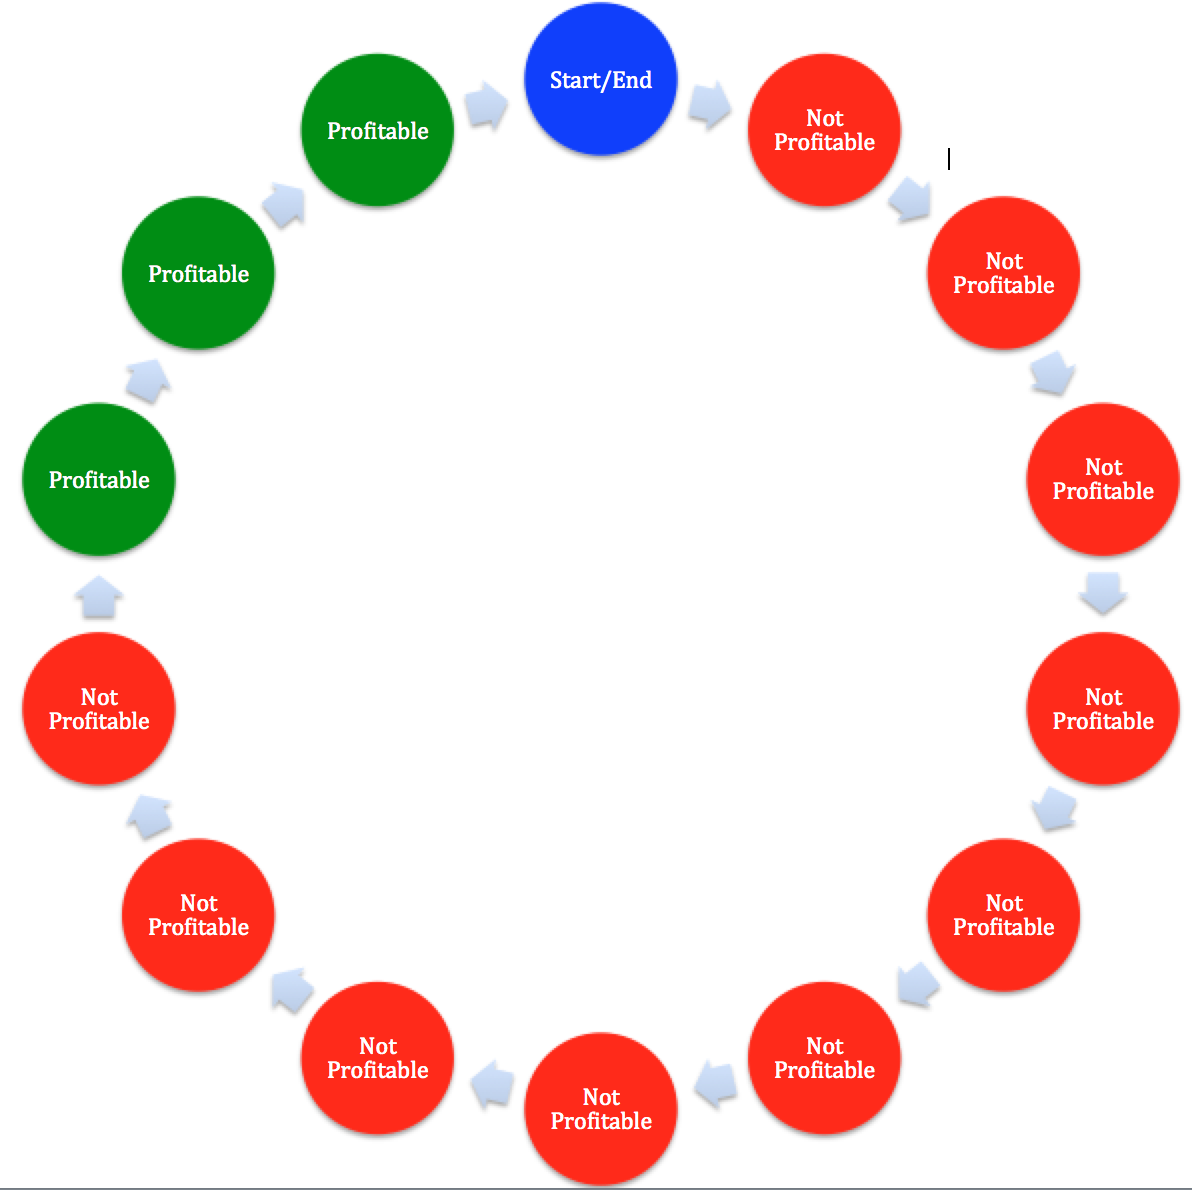
\includegraphics[width=80mm]{AlgorithmIdea.png}
\end{figure}
The Late Item Collection algorithm came to light by the acknowledgement of the following heuristic:

\begin{center}
\emph{Items taken at the start of a tour will cost the thief more money to transport than items taken later in the tour.}
\end{center}

This acknowledgement lead to the idea that if we were to rank each item by its profitability and organise the tour such that the most profitable items were taken as late in the tour as possible, this should lead to a reasonable solution to the Travelling Thief Problem.\\
The implementation of this algorithm was broken down into 5 parts:

\subsubsection*{1. Rank Each Item}
Every item in every city is given a ranking. This ranking is based on the profit of the item versus the weight of the item.
\begin{equation}
\frac{profitOfItem}{weightOfItem}
\end{equation}

\subsubsection*{2. Fill Knapsack}
\begin{figure}[h]
\centering
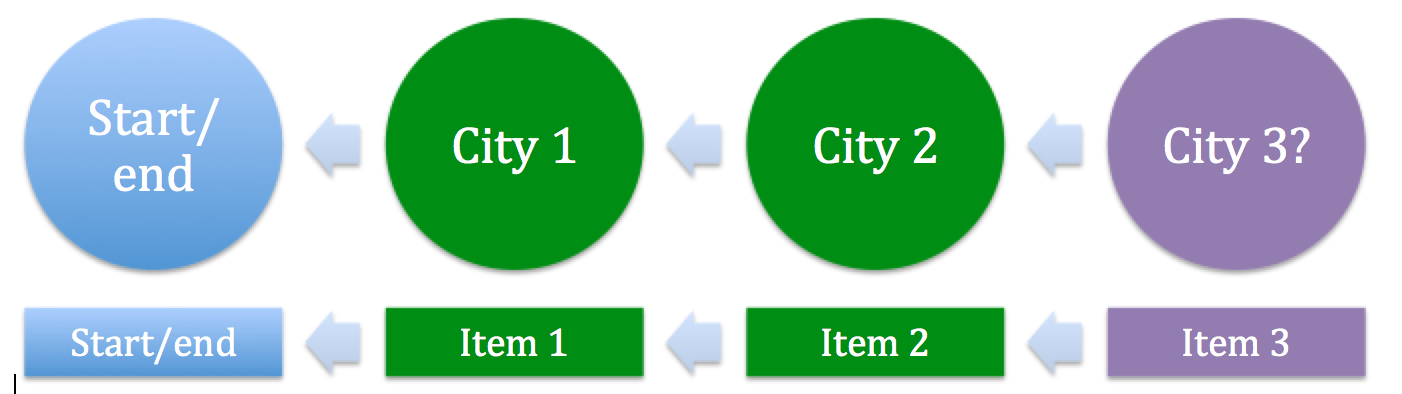
\includegraphics[width=80mm]{AddItem.png}
\end{figure}
Based on this ranking each item (in order of its rank) was tested to see if it was profitable. This was done by selecting each item (from highest ranked to lowest ranked) and then recreating the tour backwards to see if the item was profitable. For example, if an item in city 1 and 2 have already been decided to be profitable, then an item in city 3 would be tested to see if this item increases the overall profit by adding its profit and weight to the end of the chain and then evaluating the profit of this addition.

\subsubsection*{3. Split profitable/non-profitable Cities}
Based on the items taken in step two, the set of cities is now split into two subsets:

\begin{enumerate}
\item The set of non-profitable cities (visualised in red in figure 1)
\item The set of profitable cities (visualised in green in figure 1)
\end{enumerate}

\subsubsection*{3. Non-Profitable Cities}
For the set of non-profitable cities, this now becomes a simple TSP problem which is passed to our TSP solver created in assignment 1 to minimise distance travelled by the Thief (thus minimising losses).

\subsubsection*{4. Profitable Cities}
The set of profitable cities are currently ordered by the Item rank. However, this may not be the optimal tour for these cities because different permutations of this subset may yield a higher profit. For this reason I created a new selector that determined the best individual within a population based on the maximum profit. To do this I essentially reimplemented evaluate such that it would work on a subset of the problem, instead of only working on the problem space as a whole (getBestTTPSolution can be found in Population.java).

\subsubsection*{5. Recombine the subsets}
Finally, the two subsets need to be combined into the final solution. This is done by taking the best individual from step 3 and prefixing this to the best individual from step 4. Once the two subsets have been recombined into a final solution, this is then sent to TTPSolution and TTPInstance.evaluate to obtain the objective function.


\subsection*{Late Item Collection Results}
Unfortunately, the Late Item Collection algorithm does not perform very well, getting poor results on small, medium and large datasets (in fact timing out on the medium and large dataset) - splitting the problem space into two subsets, whilst a good heuristic, allows for bad results.\\
\\
Upon analysis, the reason for this is that splitting the problem into two subsets allows for a potentially good solution within the subsets themselves, but when recombined, the solution allows for expensive edge costs within the tour as a whole (as displayed in figure 3).
\begin{figure}[h]
\centering
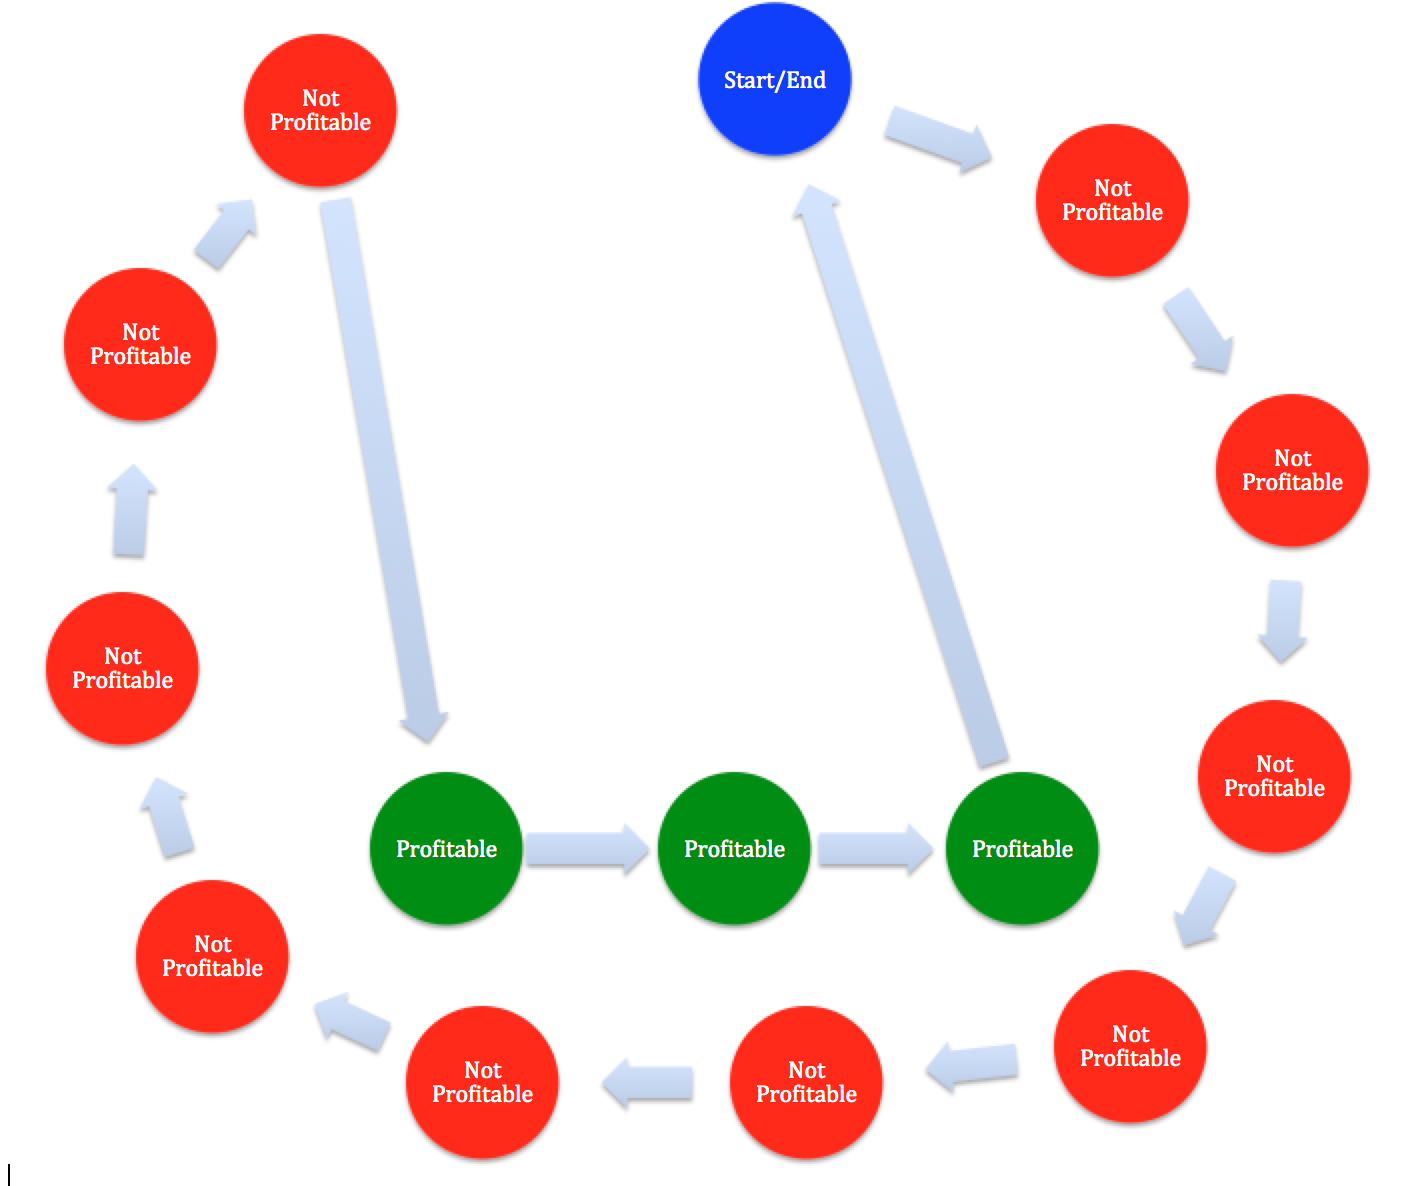
\includegraphics[width=80mm]{TheIssue.png}
\end{figure}
\\
The bulk of the time in this algorithm is spent solving the TSP, rather than filling the knapsack. Unfortunately, in the medium and large datasets, solving the TSP with a reasonable number of generations exceeds the 10 minute limit.\\

\end{document}
